\documentclass[11pt,letterpaper]{article}

\usepackage[spanish,es-tabla,es-nodecimaldot]{babel}
\usepackage{amsmath}
\usepackage[utf8]{inputenc}
\usepackage[T1]{fontenc}
\usepackage{lmodern}
\usepackage{graphicx}
\usepackage{listings}
\usepackage{anysize} 
\usepackage{fancyhdr}
\usepackage{amsmath}
\usepackage{pdfpages}
\usepackage{graphics}
\usepackage{capt-of}
\usepackage{tabularx}
\usepackage{rotating}
\usepackage{tikz}
\usepackage[colorlinks=true,plainpages=true,citecolor=blue,linkcolor=blue]{hyperref}

\marginsize{2cm}{2cm}{2cm}{2cm}
\pagestyle{fancy}
\fancyhf{Sistemas celulares}
\fancyhead[L]{\footnotesize UPIITA-IPN} 
\fancyhead[R]{\footnotesize 2TV7} 
\fancyfoot[R]{\footnotesize Tarea 2}
\fancyfoot[C]{\thepage}
\fancyfoot[L]{\footnotesize } 

\renewcommand{\footrulewidth}{0.4pt}
\renewcommand{\spanishtablename}{Tabla}
\renewcommand{\labelitemii}{$\star$}

\graphicspath{ {C:/Users/Anselmo/Documents/GitHub/upiita-SistemasCelulares/Tarea3c/imagenes} }

\begin{document}
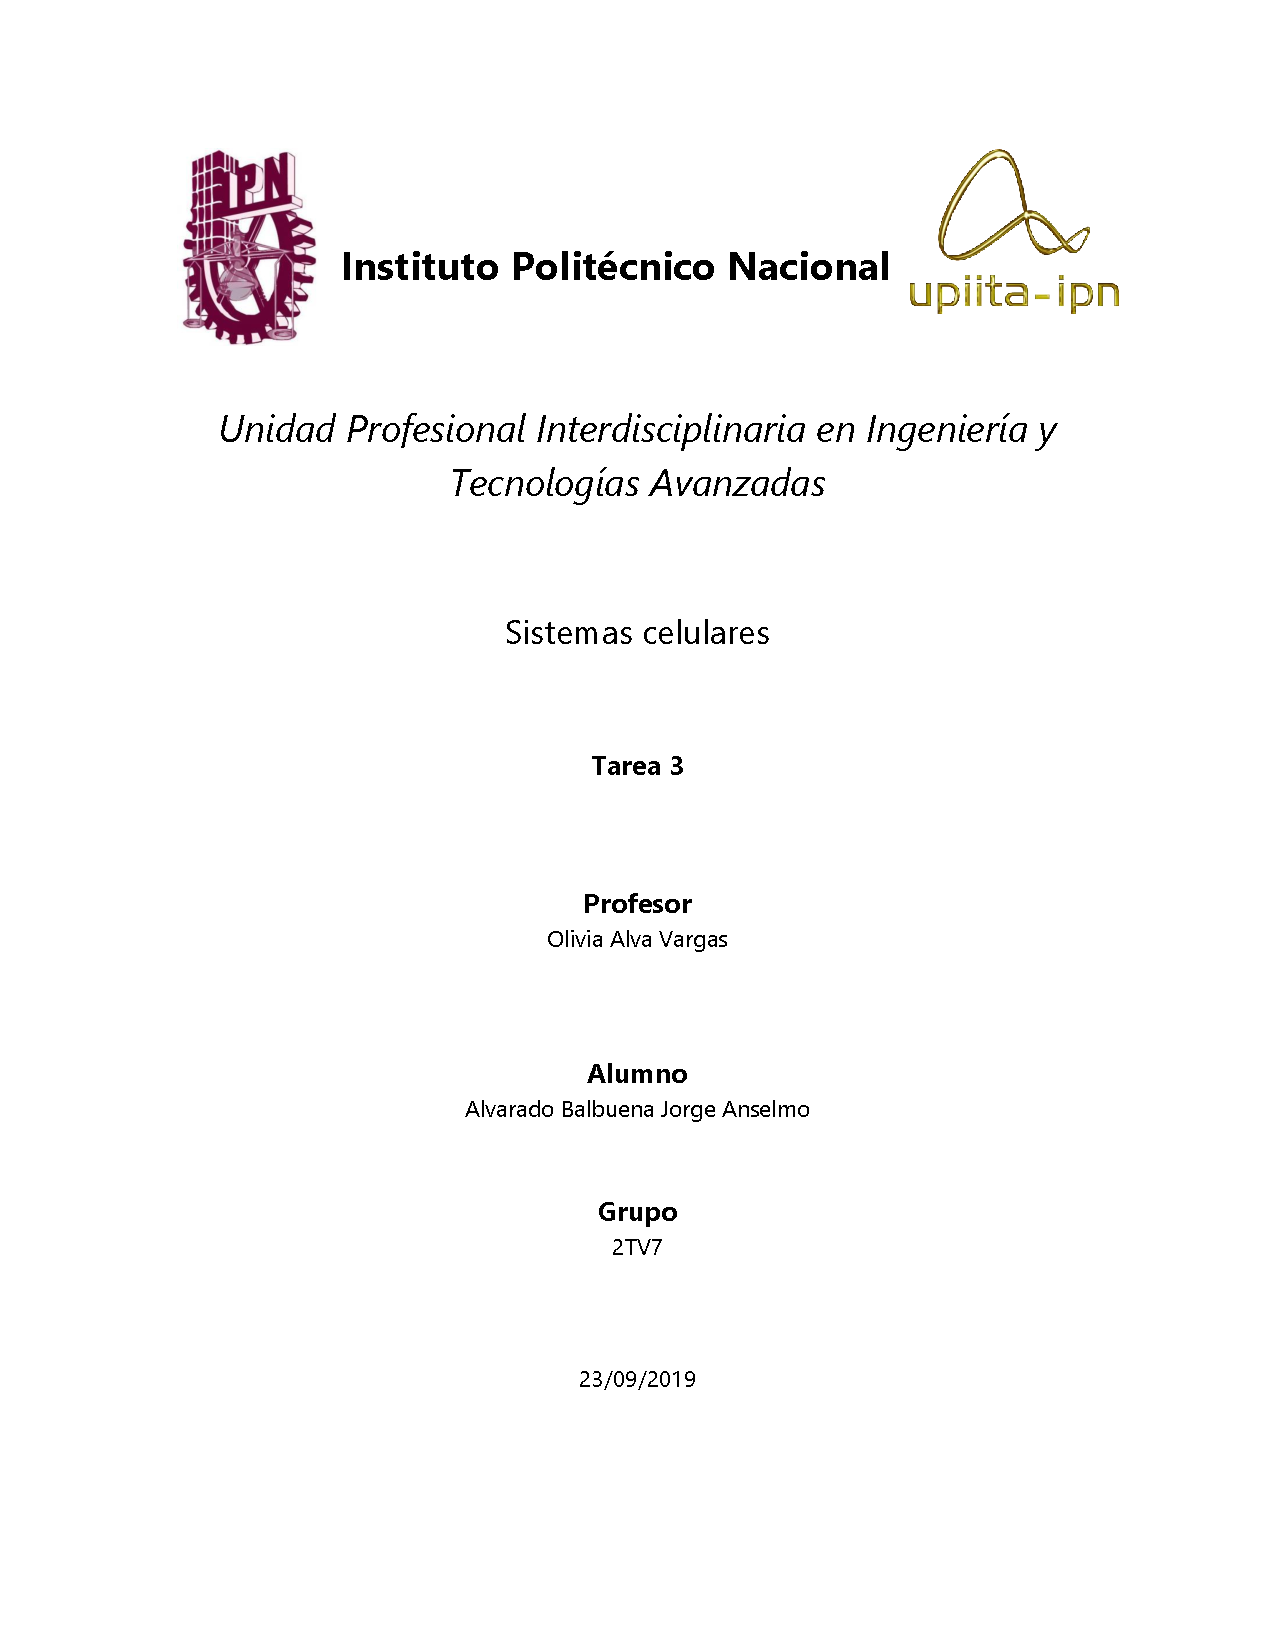
\includepdf[pages={1}]{Portada}

\newpage
\tableofcontents
\listoffigures
\listoftables


\newpage
\section{Antecedente}
\subsection{Distribución de frecuencias}
Para este estudio se tomara la distribución de frecuencias realizada en el análisis 
anterior. La distribución se muestra en la siguiente tabla. 
\begin{table}[ht]
    \centering
    \begin{tabular}{|l|l|l|l|l|}
    \hline
    Clúster & Célula & Sector & Número de canales & Canales \\ \hline
    1 & 1 & 1 & 95 & [1,31] \\ \hline
    1 & 1 & 2 &  & [32,63] \\ \hline
    1 & 1 & 3 &  & [64,95] \\ \hline

    1 & 2 & 1 & 95 & [96,127] \\ \hline
    1 & 2 & 2 &  & [128,159] \\ \hline
    1 & 2 & 3 &  & [160,191] \\ \hline

    1 & 3 & 1 & 95 & [192,287] \\ \hline

    1 & 4 & 1 & 95 & [288,383] \\ \hline

    1 & 5 & 1 & 95 & [384,431] \\ \hline
    1 & 5 & 2 &  & [432,479] \\ \hline

    1 & 6 & 1 & 95 & [480,527] \\ \hline
    1 & 6 & 2 &  & [528,575] \\ \hline

    1 & 7 & 1 & 95 & [576,623] \\ \hline
    1 & 7 & 2 &  & [624,671] \\ \hline

    2 & 1 & 1 & 95 & [1,31] \\ \hline
    2 & 1 & 2 &  & [32,63] \\ \hline
    2 & 1 & 3 &  & [64,95] \\ \hline

    2 & 2 & 1 & 95 & [96,191] \\ \hline

    2 & 3 & 1 & 95 & [192,223] \\ \hline
    2 & 3 & 2 &  & [224,255] \\ \hline
    2 & 3 & 3 &  & [256,287] \\ \hline

    2 & 4 & 1 & 95 & [288,335] \\ \hline
    2 & 4 & 2 &  & [336,383] \\ \hline

    2 & 5 & 1 & 95 & [384,431] \\ \hline
    2 & 5 & 2 &  & [432,479] \\ \hline

    2 & 6 & 1 & 95 & [480,575] \\ \hline
    \end{tabular}
    \caption{Distribución de canales.}
\end{table}

\subsection{Cantidad de frecuencias}
Tomando la tabla anterior, se tiene lo siguiente: para los dos clústeres ($N_c$=2) 
que se tienen, hay un total de 1342 canales ($n_c$=1342).

\newpage
\section{Desarrollo}
\subsection{GSM}
GSM (Sistema global para comunicación móvil) es una red móvil digital que es ampliamente 
utilizada por usuarios de teléfonos móviles en Europa y otras partes del mundo. GSM 
utiliza una variación de acceso múltiple por división de tiempo (TDMA) y es la más 
utilizada de las tres tecnologías de telefonía inalámbrica digital: TDMA, GSM y acceso 
múltiple por división de código (CDMA). GSM digitaliza y comprime datos, luego los 
envía por un canal con otros dos flujos de datos de usuario, cada uno en su propio 
intervalo de tiempo. Opera en la banda de frecuencia de 900 megahertz (MHz) o de 1,800 MHz.
\\ \\
GSM, junto con otras tecnologías, es parte de la evolución de las telecomunicaciones 
móviles inalámbricas que incluye datos de conmutación de circuitos de alta velocidad 
(HSCSD), servicio general de radio por paquetes (GPRS), entorno GSM de datos mejorados 
(EDGE) y servicio universal de telecomunicaciones móviles ( UMTS).
\subsubsection{Composición de la red}
La red GSM tiene cuatro partes separadas que funcionan juntas para funcionar como un todo: 
el dispositivo móvil en sí, el subsistema de estación base (BSS), el subsistema de 
conmutación de red (NSS) y el subsistema de operación y soporte (OSS).
\\ \\
El dispositivo móvil se conecta a la red a través del hardware. La tarjeta del módulo de 
identidad del suscriptor (SIM) proporciona a la red información de identificación sobre 
el usuario móvil.
\begin{figure}[ht]
    \centering
    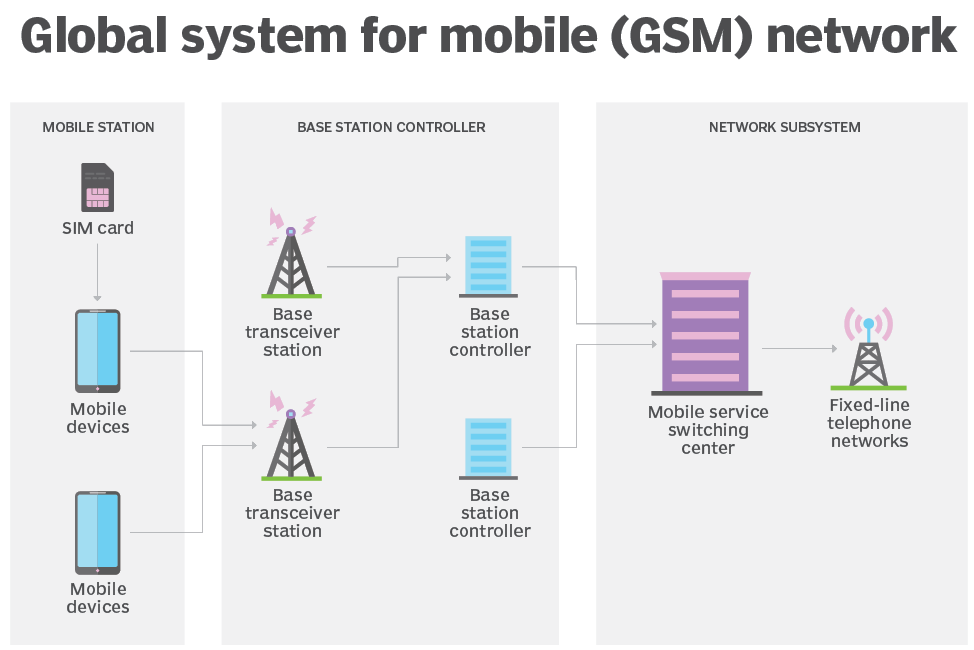
\includegraphics[width=0.75\textwidth]{imagenes/t30.png}
    \caption{Diagrama general de GSM.}
\end{figure}
\\
El BSS maneja el tráfico entre el teléfono celular y el NSS. Se compone de dos componentes 
principales: la estación transceptora base (BTS) y el controlador de la estación base (BSC). 
El BTS contiene el equipo que se comunica con los teléfonos móviles, en gran parte los 
receptores y antenas del transmisor de radio, mientras que el BSC es la inteligencia 
detrás de él. El BSC se comunica con y controla un grupo de estaciones transceptoras base.
\\ \\
La porción NSS de la arquitectura de red GSM, a menudo llamada red central, rastrea la 
ubicación de las personas que llaman para permitir la entrega de servicios celulares. 
Los operadores de telefonía móvil son dueños del NSS. El NSS tiene una variedad de partes, 
incluido el centro de conmutación móvil (MSC) y el registro de ubicación del hogar (HLN). 
Estos componentes realizan diferentes funciones, como el enrutamiento de llamadas y el 
Servicio de mensajes cortos (SMS) y la autenticación y almacenamiento de información de 
la cuenta de la persona que llama a través de tarjetas SIM.

\subsection{TDMA}
TDMA (acceso múltiple por división de tiempo) es una tecnología utilizada en la comunicación 
digital de teléfonos celulares que divide cada canal celular en tres intervalos de tiempo 
para aumentar la cantidad de datos que se pueden transportar.
\\ \\
TDMA es utilizado por el Servicio de telefonía móvil digital (D-AMPS), 
el Sistema global para comunicaciones móviles (GSM) y el Celular digital personal (PDC). 
Cada uno de estos sistemas implementa TDMA de maneras algo diferentes y potencialmente 
incompatibles. Un esquema de multiplexación alternativo a FDMA con TDMA es CDMA (acceso 
múltiple por división de código), que toma todo el rango de frecuencia asignado para un 
servicio dado y multiplexa información para todos los usuarios en todo el rango de 
espectro al mismo tiempo.

\subsection{Erlang B}
Es particularmente importante comprender los volúmenes de tráfico en las horas pico del 
día. El tráfico de telecomunicaciones, como muchos otros productos, varía a lo largo del 
día y también durante la semana. Por lo tanto, es necesario comprender el tráfico de 
telecomunicaciones en las horas pico del día y poder determinar el nivel aceptable de 
servicio requerido. La figura Erlang B está diseñada para manejar los períodos pico u 
ocupado y para determinar el nivel de servicio requerido en estos períodos.
\\ \\
Esencialmente, los diseñadores de sistemas telefónicos utilizan el modelo de tráfico 
Erlang B para estimar el número de líneas requeridas para las conexiones PSTN o las 
conexiones de cable privadas. Las tres variables involucradas son Tráfico de hora ocupada 
(BHT), Bloqueo y Líneas.

\subsubsection{Requerimiento de Erlang B}
Para lo requerimiento de Erlang B, se toma coma base principal los cambios de población 
inmigrante y emigrante referente al transporte público. Dada la cercanía del municipio 
con la terminal del transporte colectivo metro, Pantitlán. El mayor aumento en la 
población tiene como fuente el municipio de Chimalhuacán y el complemento del municipio 
de La Paz. 
\\ \\ 
Este transito se realiza por tres avenidas principales que se encuentran paralelas entre 
sí. Estas avenidas son: Av. Bordo de Xochiaca, Av. Chimalhuacán y Av. Pantitlán. 
Partiendo de la población económicamente activa en Chimalhuacán en el año 2000 que es de 
246100 de acuerdo con cifras expuestas por el INEGI. De esta población se tomará un 40\% 
de esta población dado que no necesariamente toda esta población tiene que pasar por 
este municipio para llegar al transporte metro. Para el municipio de La Paz se estima 
que hay una población de 35,226 económicamente activa. De este número se tomará el 20\%. 
Por último, para ambas poblaciones se supone que el 5\% de esa población es usaría de un 
dispositivo móvil.
\begin{figure}[ht]
    \centering
    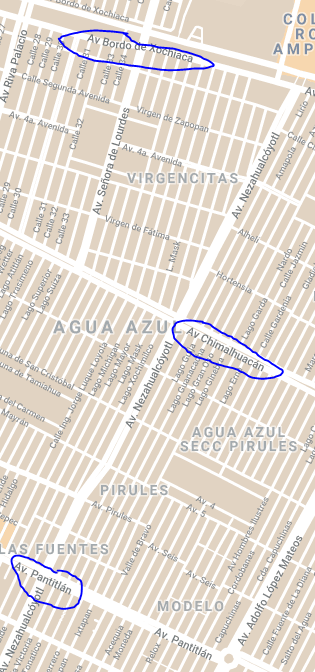
\includegraphics[width=0.4\textwidth]{imagenes/t35.png}
    \caption{Avenidas de transito.}
\end{figure}
\begin{equation}
    246100*0.4*0.05=4922 \ usuarios
\end{equation}
\begin{equation}
    35226*0.4*0.05=704 \ usuarios
\end{equation}

\subsection{Parámetros de Poisson}
Para el cambio de década se estima el aumento de población de usuarios en un 1.6\%.
\begin{equation}
    61432.7*1.6=98292.32\approx 98293
\end{equation}
Sumando la población mencionada en la sección anterior.
\begin{equation}
    98293 + 4922 + 704 = 103919 \ usuarios
\end{equation}
\\
Con el cambio del sistema AMPS a GSM, el grado de servicio aumenta de 80\% a un 99.8\%, por 
lo que el valor que será buscado en la tabla de Erlang A se calulará de nuevo. También es 
importante mencionar que los canales cambiaran por circuitos. El número de circuitos se 
obtiene con la siguiente expresión. 
\begin{equation}
    nTDMA=CH_{AMPS} \ * \ 8=1342*8=10736
\end{equation}
Se muestra en la siguiente imagen.
\begin{figure}[ht]
    \centering
    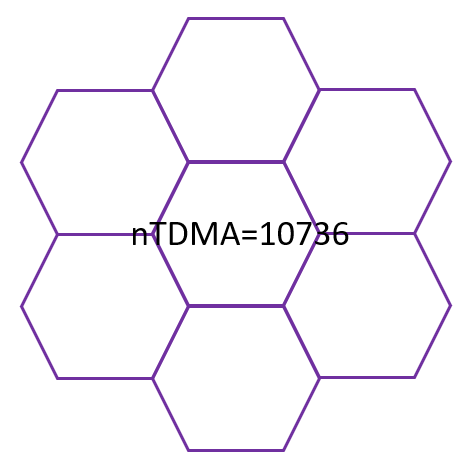
\includegraphics[width=0.4\textwidth]{imagenes/t32.png}
    \caption{Total de circuitos en el Clúster.}
\end{figure}

\newpage
\subsection{Gos 80\%}
\begin{equation}
    \frac{100-GoS}{100}=\frac{100-80}{100}=0.2
\end{equation}
$n=301 => A=371.52 \ Erlnag$
\\ 
$n_{TDMA}=1342->A_c=1,656.411 \ Erlnag$
\\ \\
$A_{TDMA}$=1,656.411
\\ \\
El número de llamadas.
\begin{equation}
    N_{TDMA}=\frac{A_{TDMA}*h_p}{\overline{t}}=\frac{1656.411*3600}{180}=33,128.22 \ llamadas
\end{equation}
\\ \\
La relación de llamadas y la nueva población.
\begin{equation}
    \frac{N}{p(00s)}=\frac{33128.22}{103919}=0.31[\frac{llamadas}{usuarios}]
\end{equation}
\\ \\
La intensidad de tráfico.
\begin{equation}
    \lambda=\frac{N}{hp}=\frac{33128.22}{3600}=9.2 \ \frac{llamadas}{seg}
\end{equation}
Conociendo $\lambda$ se calcula el espacio de arribos con la siguiente expresión.
\begin{equation}
    \frac{1}{\lambda}=\frac{1}{9.2}=0.108 
\end{equation}
La tasa de servicio $\mu$
\begin{equation}
    \mu=\frac{1}{\overline{t}}=\frac{1}{180}=5.55\overline{5} \ ms
\end{equation}
Por último se calcula la espera media de ocupaciones demoradas $t_w$ y el tiempo máximo 
de espera $\overline{t}_w$. Se propone que $t$ sea de 5 segundos. Esta propuesta tiene base en los 
requerimientos de Erlang B, más especifico, en el parámetro de tiempo máximo de espera o 
asignación. 
\begin{equation}
    t_w=\frac{t}{t_m}=\frac{5}{180}=0.02\overline{7} seg
\end{equation}
\begin{equation}
    \overline{t}_w=t_w*P(>0)=t_w*\lambda=t_w*\frac{N_{TDMA}}{hp}=0.02\overline{7}*\frac{33128.22}{3600}=0.248seg
\end{equation}
\\
Los datos obtenidos anteriormente servirán para calcular los parámetros que entrega 
la distribución de Poisson. En seguida se muestra un diagrama con los parámetros que se 
obtendrán.
\\ 
\begin{figure}[ht]
    \centering
    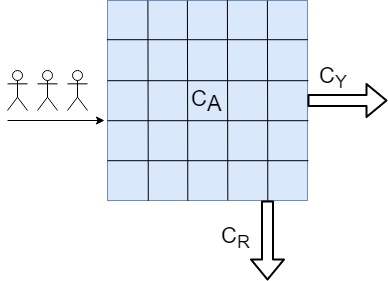
\includegraphics[width=0.7\textwidth]{imagenes/t34.png}
    \caption{Parámetros que entrega la distribución de Poisson.}
\end{figure}
\\ \\ \\
Primero se calcula las gestionadas atendidas $C_{A}$ con la siguiente expresión.
\begin{equation}
    C_A=n_{TDMA} \ * \ \lambda = 10736 * 9.2=98771.2
\end{equation}

Ahora las llamadas cursadas $C_Y$ con un Erlang B igual a 0.01.
\begin{equation}
    C_Y=C_A(1-B)=98771.2(1-0.01)=97783.488
\end{equation}

Por ultimo las llamadas rechazadas.
\begin{equation}
    C_R=C_A*B=98771.2*0.01=987.712
\end{equation}

Con la información anterior se puede obtener las gestiones efectivas.
\begin{equation}
    C_A-C_R=98771.2-987.712=97783.488
\end{equation}


\newpage
\subsection{Gos 99.8\%}
Ahora el valor de la tabla de Erlang A para un GoS 99.8\%.
\begin{equation}
    \frac{100-GoS}{100}=\frac{100-99.8}{100}=0.002
\end{equation}
$n=301 => A=264.18 \ Erlnag$
\\ 
$n_{TDMA}=1342->A_c=1177.839 \ Erlnag$
\\ \\
$A_{TDMA}$=1177.839
\\ \\
El número de llamadas.
\begin{equation}
    N_{TDMA}=\frac{A_{TDMA}*h_p}{\overline{t}}=\frac{1177.839*3600}{180}=23556.781 \ llamadas
\end{equation}
\\ \\
La relación de llamadas y la nueva población.
\begin{equation}
    \frac{N}{p(00s)}=\frac{23556.781}{103919}=0.226[\frac{llamadas}{usuarios}]
\end{equation}
\\ \\
La intensidad de tráfico.
\begin{equation}
    \lambda=\frac{N}{hp}=\frac{23556.781}{3600}=6.543 \ \frac{llamadas}{seg}
\end{equation}
Conociendo $\lambda$ se calcula el espacio de arribos con la siguiente expresión.
\begin{equation}
    \frac{1}{\lambda}=\frac{1}{6.543}=0.152 
\end{equation}
La tasa de servicio $\mu$
\begin{equation}
    \mu=\frac{1}{\overline{t}}=\frac{1}{180}=5.55\overline{5} \ ms
\end{equation}
Por último se calcula la espera media de ocupaciones demoradas $t_w$ y el tiempo máximo 
de espera $\overline{t}_w$. Se propone que $t$ sea de 5 segundos. Esta propuesta tiene base en los 
requerimientos de Erlang B, más especifico, en el parámetro de tiempo máximo de espera o 
asignación. 
\begin{equation}
    t_w=\frac{t}{t_m}=\frac{5}{180}=0.02\overline{7} seg
\end{equation}
\begin{equation}
    \overline{t}_w=t_w*P(>0)=t_w*\lambda=t_w*\frac{N_{TDMA}}{hp}=0.02\overline{7}*\frac{23556.781}{3600}=0.176seg
\end{equation}
\\ 
Los datos obtenidos anteriormente servirán para calcular los parámetros que entrega 
la distribución de Poisson. En seguida se muestra un diagrama con los parámetros que se 
obtendrán.
\\ 
\begin{figure}[ht]
    \centering
    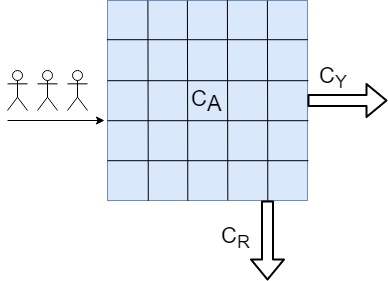
\includegraphics[width=0.7\textwidth]{imagenes/t34.png}
    \caption{Parámetros que entrega la distribución de Poisson.}
\end{figure}
\\ 
Primero se calcula las gestionadas atendidas $C_{A}$ con la siguiente expresión.
\begin{equation}
    C_A=n_{TDMA} \ * \ \lambda = 10736 * 6.543=70245.648
\end{equation}

Ahora las llamadas cursadas $C_Y$ con un Erlang B igual a 0.01.
\begin{equation}
    C_Y=C_A(1-B)=70245.648(1-0.01)=69543.191
\end{equation}

Por ultimo las llamadas rechazadas.
\begin{equation}
    C_R=C_A*B=70245.648*0.01=702.456
\end{equation}

Con la información anterior se puede obtener las gestiones efectivas.
\begin{equation}
    C_A-C_R=70245.648-702.456=69543.19
\end{equation}

\newpage
\section{Conclusión}
La población estimada para la realización de este estudio y la cual se tiene registrada 
en los inicios de la década de los 2000s varia bastante. En seguida se muestra una 
tabla mostrando la evolución demográfica del municipio.
\begin{figure}[ht]
    \centering
    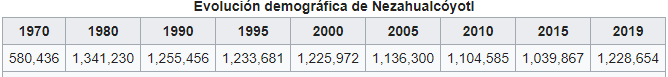
\includegraphics[width=0.9\textwidth]{imagenes/t31.png}
    \caption{Evolución demográfica del municipio de Nezahualcóyotl.}
\end{figure}




Para estos datos el cambio de AMPS a GSM resulta en que el servicio se clasificaría como 
insuficiente. Aunque hay factores demográficos y socioeconómicos que hay que temar en 
cuenta. El primero de ellos, es considerado como uno de los municipios con mayor densidad 
poblacional. Así que si se pusiera en uso el sistema GSM en horarios de noche-madrugada-mañana, 
el sistema dejaría sin servicio a un gran número de la población. Estos suspuestos pueden cambiar 
en la realidad. 
\\ \\
Pero ¿por qué se menciona 
en concreto este horario? Como gran parte de los municipios del Estado de México que se 
encuentra alrededor de la Ciudad de México, también llamada zonza conurbada, es considerada 
una ciudad dormitorio por su carácter mayoritariamente residencial. Esto quiere decir que 
la mayor parte de la población económicamente activa trabaja en otra zona, para en este caso 
particular, la Ciudad de México. Otra razón por la cual mencionar este horario, es que la 
población económicamente activa mayor a 30 años del municipio es de aproximadamente un 85.21\%. 
\\ \\
De este porcentaje el 70,77\% son hombres y 39,52\% son mujeres. Por lo que la noche, cuando 
un gran número de población regresa, la madrugada, cuando la mayor parte de la población se 
encuentra en la zona y la mañana, cuando esa población que regreso vuelve a salir, son los 
periodos en lo que el sistema tiene una mayor demanda. Por lo que esto deja al día corriente 
como el horario cuando mejor servicio podría proporcionarse a la población. Se tiene que 
señalar que en caso de el suceso de una situación extraordinaria el sistema podría presentar 
deficiencias dejando a un gran numero de usuario sin servicio, aun tomando en consideración 
el reinicio del uso de los circuitos cada hora.
\end{document}

\end{document}